\documentclass[a4paper, 11pt]{report}
\usepackage[T1]{fontenc}
\usepackage[utf8]{inputenc}
\usepackage{times}
\usepackage[libertine]{newtxmath}
\usepackage{graphicx}
\usepackage[pdfa]{hyperref}
\usepackage{color}
\usepackage[a4paper, inner=0.5cm, outer=0.5cm, lmargin=2.6cm, rmargin=2.6cm,
tmargin=2.0cm, bmargin=2.1cm]{geometry}
\usepackage{listings}
\definecolor{dkgreen}{rgb}{0.1,0.5,0.1}
\definecolor{greengray}{rgb}{0.32,0.57,0.32}
\definecolor{orange}{rgb}{0.96,0.42,0}
\definecolor{lightblue}{rgb}{0,0.28,0.95}
\definecolor{background}{rgb}{0.995,0.995,0.995}
\lstset {
	frame=tb,
	language=java,
	aboveskip=3mm,
	belowskip=3mm,
	showstringspaces=false,
	columns=flexible,
	basicstyle={\small\ttfamily},
	numbers=none,
	backgroundcolor=\color{background},
	numberstyle=\tiny\color{drkgeen},
	keywordstyle=\color{lightblue},
	commentstyle=\color{greengray},
	stringstyle=\color{orange},
	breaklines=true,
	breakatwhitespace=true,
	tabsize=3
}

\begin{document}
\title{Computer Networks 2 and Introduction to Cybersecurity}
\author{Marco Sgobino}
\maketitle
\tableofcontents

\part{Transmission Control Protocol internals}

\chapter{Basics}

\section{Brief recap of TCP}
TCP is a procotol that has the following properties,

\begin{itemize}
	\item allows \emph{connection between processes};
	\item is \emph{connection-oriented}: before transmitting data, a
		connection must be established \--- this is different to what
		IP protocol does in network layer, since in IP protocol there
		is no concept of connection, and messages are exchanged in
		packets;
	\item is \emph{reliable}: it assures all segments are correctly
		delivered through use of \emph{ACK} mechanism, and \textbf{at
		most once} \--- again, this is different to IP layer, since IP
		packets are unreliable and there is no guarantee that they will
		be delivered, let alone in their correct ordering;
	\item offers a \emph{sliding window} mechanism for congestion control
		and stream control. This assures read and send buffers are
		well-optimized in both sender and receiver \--- this feature is
		much important since it allows fine-tuning the connection and
		avoiding waste of resources;
	\item is \emph{byte-oriented}: the byte stream is fragmented into
		multiple segments, and composed again after getting to
		destination \--- in this manner, huge payloads can be reliably
		delivered in multiple segments, each one having the correct
		order to the application.
\end{itemize}

The logical structure is the following one: there are two entities, client and
server. The client first authenticates to the server; after that, the server
opens a connection and client executes the send-receive loop. Both server and
client create a \emph{socket} $s$ (a UNIX-like file abstraction), and the
client connect $s$ to IP-srv, port-srv. The communication takes place on $s$ by
means of application protocol (applications will exchange data each other). The
connection is said to be \emph{reliable}: losses and packet loss are carefully
managed, and segments\footnote{\emph{Segments} refer to the particular kind of
package that TCP protocol exchange. Usually, in literature one could find the
term package referring to TCP segments; while this is not fully correct, it may
be acceptable when there is no ambiguity.} arrive in the same order as they are
sent.

A very simplified pseudo-code at client's side for TCP is as follows,

\begin{verbatim} int s; s := socket(...); 
connect(s, IP-srv, port-srv,...); 
...
send (s, msgl, ...); 
... 
msg2 := receive(s,...); 
... 
\end{verbatim}

where the notation \emph{...} denotes possibly code in between two
instructions.

The logical structure at server side is quite different. A server creates
a socket $s1$, chooses a port number to bind to that socket, then it declares
willingness to accept connections on $s2$, and finally it awaits for connection
requests on $s2$. Basically, it creates two different sockets, the first to
accept a new connection, and the second one to actually manage the connection.
A server usually remains on \emph{sleep} until a connection is requested.

\begin{verbatim} 
s1 := socket(...);
bind(s1, portsrvm ...);
listen(s1,...);
s2 := accept(s1,...); // another socket 
... 
msg1 := receive(s2,...);
...
send(s2,msg2,...);
... 
\end{verbatim}

In TCP, communication is \emph{bidirectional}, with a pattern that depends on
the application protocol. The send-receive patterns heavily depend on the
application itself \--- browser send-receive sequences are very different from,
let's say, an e-mail client send-receive sequence. There is no guarantee that
two different application protocols will exchange a similar amount and kind of
TCP messages.

\subsection{TCP Implementation}

There are many differences between TCP and IP, set aside their abstraction
layer. IP operates between \emph{nodes}: it is \emph{connectionless},
\textbf{unreliable}, and is \emph{message-oriented}. The Maximum Transmission
Unit size of an IP packet is $MTU = 64KB$. TCP lies on top of IP, adopting
coutermeasures to overcome the unreliable aspects of IP.

TCP layers communicate between themselves in terms of \emph{segments}. A
segment is a \emph{message between TCP layers}, and contains a \emph{TCP
header} and \--- eventually \--- data \emph{payload}. Payload can either be $0$
bytes long or carry some information (wanted by the application layer). An
important property is that \emph{a TCP segment must be small enough to fit in a
single IP packet}, hence IP header and TCP segment size should be no greater
than $64KB$, the MTU of an IP packet.

A segment is thus composed by a IP header, whose payload is a TCP segment. The
TCP segment is in turn composed by a TCP header, followed by eventual
application data. Usually, IP header size is usually $20$ bytes, as well as TCP
header that is $20$ bytes. The IP datagram can be greater up to $64KB$, with
the first $40$ to $50$ bytes reserved to headers.

Segments can carry portions of data (for instance, in a video stream many
segments should be sent to client in order to carry enough information and let
application layer reconstruct the video correctly). For this reason, in
application layer, one application message could correspond to \emph{many
segments} in TCP layer, in \textbf{both} directions. In fact, at TCP level
multiple segments are usually required in order to send a single
application-level message. Each TCP layer represents a connection as (<id>,
<state>). The <id> is the <IP-local, port-local, IP-remote, port-remote>, while
the <state> refers to the state of the TCP connection. Conceptually there is a
single table storing both <id> along with connection <state>.

IP addresses are extracted from the IP header, while port numbers are extracted
from TCP header. Packets are thus sorted accordingly. The connection <state>
includes information on the \emph{Maximum Segment Size} (MSS), which is the
maximum size of the \emph{data part} of a segment that the other part is
willing to achieve. The MSS is negotiated upon connection opening \--- this
value is, in practice, identical in both direction and is not arbitrary. In
most cases and for historical reasons, there are only $2$ possible values that
depend whether the connection:

\begin{itemize}
    \item lies on different networks (through internet), MSS is $536$ bytes
        (MTU=576), that is the maximum segment size that can fit in the
        smallest possible packet;
    \item lies on the same network (for example, ethernet), MSS is $1460$ bytes
        (MTU=1500), which corresponds to ethernet MTU minus the IP header and
        TCP header.
\end{itemize}

The core idea is that each segment must be \emph{sufficiently small} to fit in
one packet along the full path, in order to prevent fragmentation.

\subsubsection{Establishing a TCP Connection}

At the beginning of a TCP connection, $3$ segments are needed, while $2$
segments are needed to close it.

FIXME DNS -> To forge it, must change IP address to
response AS WELL AS copying Transaction ID of request

\section{TCP Architecture}

TCP has many different implementations, depending mostly on OS of choice.
Several variants of its components have been written, with many of them largely
optional. TCP works in segments. Execution flow at application level works
independently and unpredictably with respect to the TCP-level flow. When an
application sends something, multiple TCP packages must be exchanged. The
sequence of bytes will be copied to a buffer (sliding window) and the
\emph{send()} function is, for example, invoked \--- the time in which a
segment is sent is \emph{unpredictable}, \emph{unrepeatable} and depends on
many things. This means that application cannot \emph{deterministically
predict} the exact time in which the transmission will occur \--- instead, the
TCP layer will deliver the payload at a specific time determined by the
protocol\footnote{However, many more effects can concur: for instance, the
Operating System may not be ready to send a segment, or may be busy with other
resources.}.

On TCP, many events can provoke a transmission:

\begin{itemize}
    \item application invokes \emph{send()} \--- in this case, the data in
        send's call argument will be inserted into the proper transmission
        buffer, and it will be transmitted somewhere in the (immediate) future;
    \item application invokes \emph{receive()} \--- this way, we will see in
        detail that the TCP protocol provides a \emph{response} that
        \emph{acknowledges} the receipt of a segment;
	\item TCP layer \emph{receives a segment} \--- the same as above;
	\item a \emph{timeout} occurs;
\end{itemize}

Each of the above will trigger a transmission either immediately or
\emph{withing a maximum predefined time} (in the case of a timeout, for
instance). When a TCP layer is touched from above or below, \textbf{it reacts
by transmitting a segment}. Transmission may occur \emph{even if there is no
useful data to transmit} (e.g. the transmission buffer is empty) \-- in that
case, a segment will only carry the header, which has information useful to the
protocol itself. Upon transmission, TCP may deliver a varying number of bytes,
ranging from empty up to a number of bytes \emph{larger than Maximum Segment
Size} ($536$ in Internet network, $1460$ for same Ethernet network). To send a
huge paylod, the TCP protocol \emph{fragments} it before delivery, resulting in
multiple segments delivered in sequence. It is not uncommon that $2$ or $3$
segments are initially delivered before the acknowledgement.

\begin{table}[ht]
\centering
\begin{tabular}{cc}
CPU Cycle & $0.3 ns$ \\
Main Memory Access (DRAM) & $120ns$ \\
SSD & 50-150 $\mu s$ \\
HHD & $10 ms$ \\
Internet, San Francisco to New York & $40ms$
\end{tabular}
\caption{Some interesting metrics. Notice the order of magnitudes differences
between CPU cycles and network delays.}\label{tab:SomeMetrics}
\end{table}
\bigskip

The TCP protocol starts with slowly sending segments, increasing the exchange
speed as the time goes on. Acceleration mainly depends on the timing of
\emph{received} segments, by looking at the metrics of confirmation packets
from receiver. As the sender acknowledges that the receiver is able to keep up
with the increasing transmission speed, it raises the delivery speed.

\subsection{The \emph{send()} system call}

The system call \emph{send()} processes the data transmission through the
network. The \emph{send} function passes a memory buffer contained in
application space (address, length), and copies bytes from transmission memory
buffer in application space to transmission memory buffer in TCP layer (called
\textbf{TX-buffer}).

\begin{lstlisting}
public void write(byte[] b)
	throws IOException
\end{lstlisting}

Send is first invoked by application level. Buffer at application layer is then
copied to the TCP transmission buffer, to be sent immediately or later. New
invokations of \emph{send()} will copy data in TCP buffer \textbf{after} the
data that is already present. 

\subsection{The \emph{receive()} system call}

When data reaches the receiver, the data is copied into a receiving buffer
(RX-buffer). The receiver buffer stores all received bytes and is flushed only
when the application invokes \emph{receive()}. The function
\emph{receive()} copies (at least a portion of) the receiver buffer into the
application buffer by means of passing a buffer of \emph{address} and
\emph{length}. Function receive() copies bytes without exceeding the size of
the buffer (\emph{length}) and it returns how many bytes are copied. As
argument, receive() also takes the number of bytes to get from the TCP
receiving buffer.

There are three possible outcomes for the receive() call:

\begin{itemize}
	\item if the receive buffer is empty, the application is suspended and
		the process is put to sleep;
	\item if more than \emph{length} bytes are available, a
        \emph{length} number of bytes is fetched and delivered to the
        application;
	\item if less than \emph{length} bytes are available, all available
        bytes are copied since they are less than the maximum deliverable
        value.
\end{itemize}

\subsection{Sending N bytes}

Suppose to send $N$ bytes with $K$ consecutive \emph{send()} invocations. How
many segments will be exchanged? How many transmission events?

As a first approximation, the number of transmitted segments will roughly be
$$num = \frac{N}{MSS} + 1,$$ with the last segment $+1$ smaller than the
previous ones. Things, however, can be much more complex due to packet loss and
retransmissions. Recall that the number per se is not predictable and not
repeatable (TCP is byte-oriented, and will send a proper number of segments).

\section{Sequence numbers}

IP protocol is \emph{unreliable} (packets can be lost, duplicated, or delivered
in different order from which they were sent), each data byte is implicitly
identified by a $32$ bit \textbf{sequence number}. The association is implicit
\--- the sender applies a sequence number to a segment, and the receiver uses
that information to reconstruct the original order of segments. Segments are
then reconstructed, and the data assembled as it originally was.

There are several sequence numbers. \emph{snd.User} is the variable carrying
the value of the next byte the \textbf{application} will send.
\emph{snd.Next} is the variable carrying the value of the next byte that the
\textbf{TCP layer} will transmit \--- its value is contained in the TCP header
(initial byte of the sequence, of course). Basically, \emph{snd.User} refers
to the next byte that will be filled by the invocation of \emph{send()},
while \emph{snd.Next} is the next byte yet to transmit by the TCP layer. The
sequence number of application level must be computed from other information.
\footnote{An important detail is that \textbf{sequence numbers are 32-bit integers}.
Therefore, there may be a \emph{wrap-around} in an overflow-like fashion. TCP
should internally handle these comparisons in a proper manner.}

In short,

\begin{itemize}
	\item \emph{snd.Next} is the boundary between transmitted data and
		yet-to-transmit data;
	\item \emph{snd.User} is the boundary between in TX-buffer data (data
		sent by application) and not-yet-associated bytes.
\end{itemize}


\begin{figure}[b]
        \centering
        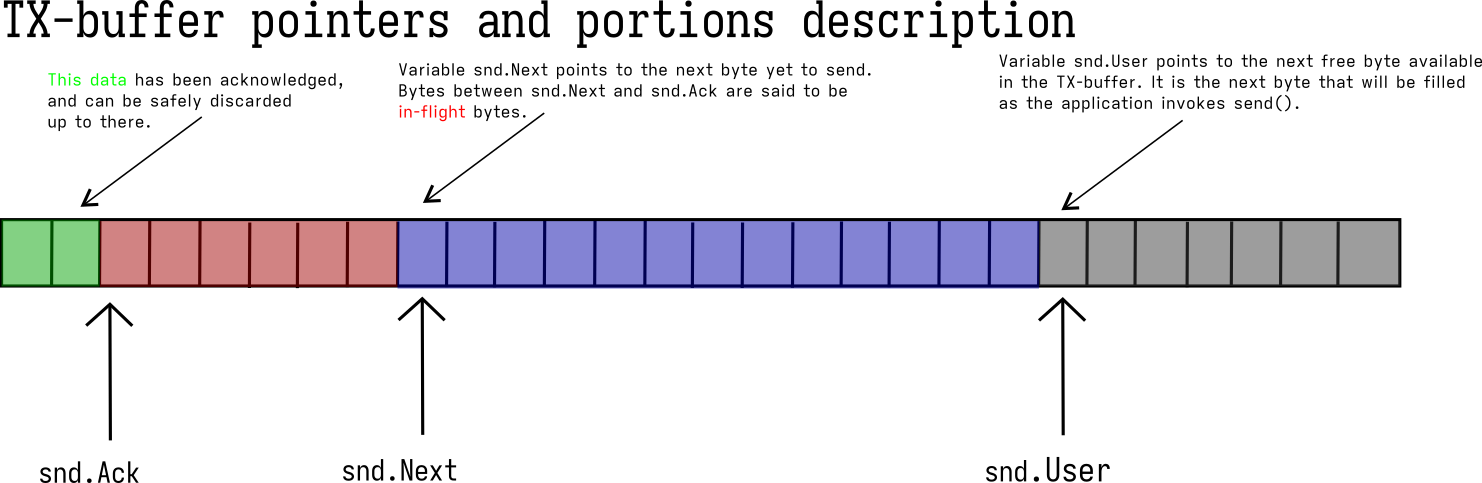
\includegraphics[ width=1.0\linewidth, height=\textheight, keepaspectratio]{./pics/tcp/TxBuffer.png}
	\caption{TX-Buffer and its flags \emph{snd.Ack}, \emph{snd.Next} and \emph{snd.User}.}
        \label{fig:TxBuffer}
\end{figure}

From the receiver's point of view, there is a variable, \emph{rcv.Next}, that
is the boundary between content of RX-buffer and not-yet-received data (right
boundary of the data currently in buffer). The variable \emph{rcv.Next} is
similar to the variable \emph{rcv.Next} in the sense that it points at the
next byte yet to receive. Only packets having expected sequence number are
collected and put in the buffer. There is the case where some packet has new
parts of information and sequence numbers not collected: in that case the
incoming segment will still be collected, with duplicated bytes thrown away.
There may be two reasons for packet duplications: IP duplication, and TCP
sender retransmission because it thought it was lost. TCP stores packets in
buffer until acknowledgement has been received, since they could be
retransmitted in the immediate future.

\begin{itemize}
	\item \emph{rcv.Next} points at the next byte that is not yet being
		received;
	\item \emph{rcv.User} points to the next byte to be received by the
		application. After \emph{receive()} invokation by the
		application, all delivered to the application bytes can now be
		deleted, since there are no retransmission needs. 
\end{itemize}

\begin{figure}[b]
        \centering
        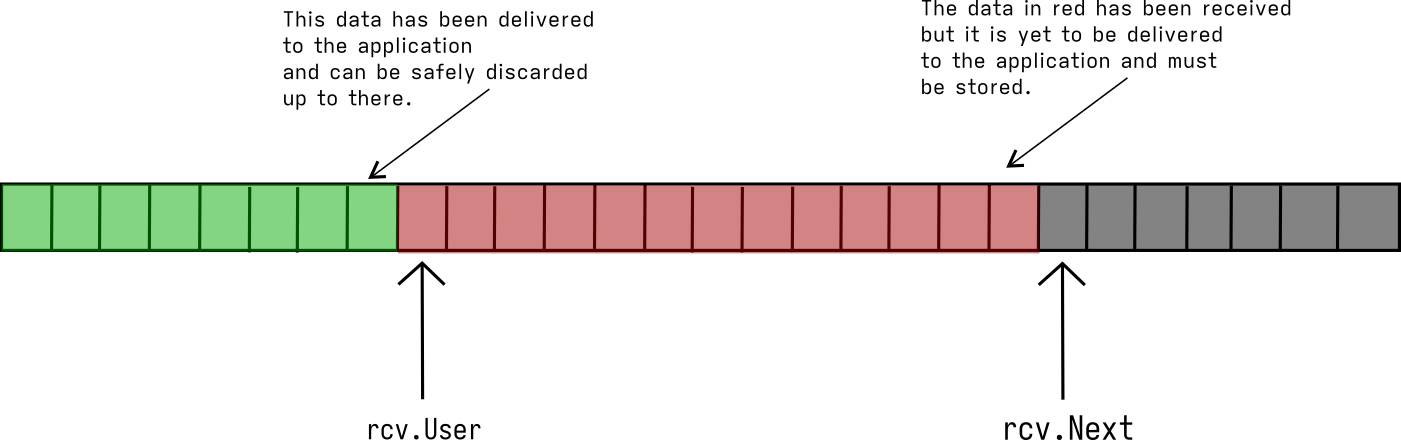
\includegraphics[ width=1.0\linewidth, height=\textheight, keepaspectratio]{./pics/tcp/RxBuffer.png}
    \caption{RX-buffer and its flags. Notice that RX-buffer only uses two flags
    instead of three (no ACK flag needed).}
        \label{fig:RxBuffer}
\end{figure}




\section{Handling duplicates and loss}

IP is an unreliable protocol. This means that \emph{packets can be loss}.
Necessary mechanisms are

\begin{itemize}
	\item \textbf{retransmission};
	\item \textbf{acknowledgement}, which is a kind of \emph{notification
		of receipt}, in order to be sure that the receiver has received
		all the data we sent them.
\end{itemize}

Acknowledgements are a mechanism that assures receipt of a message by
notifications. Every header of a segment contains the sequence number of
\emph{snd.Next}. Every segment also \emph{carries an information regarding
the bytes that are received}: the \textbf{acknowledgement number}, which tracks
the state of the RX-buffer by the pointer \emph{rcv.Next}. This way, having
both sequence number and acknowledgement number, one can successfully track the
state of a TCP connection. When sending a TCP segment, both sequence number and
acknowledgement number are sent, so that the receiver can reconstruct the state
of the sender RX-buffer.

A fifth variable is needed: \emph{snd.Ack}, which \emph{points to the byte in
TX-buffer that are both transmitted and acknowledged}. This variable is only
increased upon receiving data (for instance, upon receiving a sequence with a
greater ACK number from the sender). Data before \emph{snd.Ack} pointer can
safely be discarded. Acknowledgements are crucial to a TCP connection, in order
to guarantee \textbf{reliability} of a connection (TCP is connection-oriented).
Therefore, transmission is always necessary even if TX-buffer is empty. That
case, no payload will be transmitted, only information in header is sent
(increasing acknowledgement number). 

Data bytes between pointers \emph{snd.Ack} and \emph{snd.Next} is said to
be \emph{in flight} data. These bytes have been transmitted but not yet
acknowledged.


\section{Delayed Acknowledgement}

\emph{Delayed Acknowledgement} is a famous TCP algorithm. It is pretty
straightforward:

\begin{quote}
Upon receiving a segment, if delayed-ack timer $T$ has previously been set,
transmit immediately. Else, set the delayed-ack timer $T$ to a value.
\end{quote}

Delayed-ack timer value depends on the operating system:

\begin{itemize}
	\item RFC suggests $T = 500ms$;
	\item Windows has $T = 200ms$;
	\item Linux in general has $T = 40ms$;
	\item RHEL sets $T = 4ms$.
\end{itemize}

If there is not much data to transmit, it will be likely that the timer $T$
will expire. If the other part is sending a lot of data, the contrary will be
more likely to occur, breaking the awaiting. \emph{In order to help the other
part, acknowledges will be delivered as soon as a second segment is received}.
The core idea is to both help the other end and minimize the number of segments
to be sent. In fact, a delay time $T$ assured to save sending some segments, a
feature that historically was of a crucial importance.

\section{Retransmissions}

The connection state includes three more variables:

\begin{itemize}
	\item a \textbf{retransmission timer};
	\item a \emph{variable that describes the duration of retransmission
		timer}, the \textbf{RTO};
	\item a \textbf{retransmission counter}.
\end{itemize}

The algorithm is as follows:

\begin{quote}
Upon transmitting segment S, the counter is cleared and set to $0$, with the
timer set to the RTO value. Upon receiving an ACK, \emph{snd.Ack} is set to
the maximum value between \emph{snd.Ack} and \emph{segment.Ack}. If
\emph{snd.Ack == snd.Next} the timer is switched off.

When timer expires, the counter is incremented and if the counter has not yet
reached a \emph{MAX\_COUNT} value, the segment is retransmitted. However, this
time the timer value is set to RTO but \emph{RTO = 2 * RTO}. Only in-flight data
should be retransmitted (and all of it after timer expires). Basically, data
for which we are sure that it has been received, should not be retransmitted in
case the timer expires.

When counter reached \emph{MAX\_COUNT} value, connection is closed.

A particular condition is when an ACK arrives for a portion of the data that
has been sent. In that case, the timer resets (the receiver has responded) and
the sender awaits ACK for missing segments.
\end{quote}

Windows closes connection after $5$ failed attempts, Linux after $15$. It is
simple to realise that there may be a lot of unnecessary retransmissions. The
timer can, for instance, run out too soon for the acknowledgement to reach the
sender. Unnecessary retransmissions are a waste of resources, a fundamental
problem. The reason could be one of those:

\begin{itemize}
    \item segments are \emph{lost};
    \item segments \emph{which ACK are lost};
    \item RTO was set to a \emph{too small value}.
\end{itemize}

Thus, RTO should be set to an appropriate value, since a too short value leads
to high overhead and possibly many unnecessary retransmissions, while a too
long value results in high latency and possibly a slow connection. RTO value is
basically a trade-off between few retransmissions and fast connection. RTO
should be set \textbf{dinamically}. The RTO should be slightly greater than the
\emph{RTT} (round-trip-time), and it is an idea from Jacobson algorithm. This
is of a crucial importance for TCP to work. Initial RTO value is heuristical,
and varies from one OS to another. Linux and Window start from same value,
macOS use a different value, and so on.

\section{Multiple default gateways}

More default gateways could be added to a single node. Reasons to add more than
one default gateway all boil up to \emph{failure avoidance}. To know whether a
gateway has stopped working, a heuristic TCP algorithm tries to detect a gateway failure:

\begin{quote}
	if the number of retransmissions is greater than a \emph{MAX\_COUNT}
	divided by 2 number, the \emph{connection} changes its default gateway.
	Moreover, if the number of connections that changed default gateway is
	greater than the number of open connections divided by 4, the \emph{IP
	layer} changes the default gateway. This last feature speeds up
	reconfiguration of early connections that still have to make some
	retransmission attemps.
\end{quote}

Basically, each connection can autonomously choose its own gateway, but the IP
layer is able to force any \--- new or already present \--- connection to use a
different default gateway.

\section{Gaps in RX-buffer}

Suppose that 4 segments are sent, and the second one has been lost. In this
case, the receiver received all segments except the second one, however it has
no method to inform the sender to retransmit only the second segment. Sending
ACK for only the first segment would result in unnecessary retransmission of
segments 3 and 4, which were correctly received. The receive buffer could end
up having some \textbf{gaps}, missing bytes that are supposed to be received.
The solutions are \emph{Selective Acknowledgements} (SACK), a special kind of
acknowledgements that carry both \emph{left and right sequence number edges} of
each out-of-order \textbf{block} in RX-buffer, this way avoiding unnecessary
retransmissions. SACK protocol must be supported by both members of a
connection. SACK is very convenient, since many segments can be lost when a
sender tries to deliver dozens of segments at once. This way, TCP can achieve
\emph{efficient handling} of the connection.

Of course, out-of-order segments could still lead to gaps in RX-buffer. In this
case, unnecessary retransmissions are unavoidable when an out-of-order segment
reaches the receiver too late (however, SACK reduces a lot the burden to the
sender since only missing segments should be selectively sent).

\section{Operating System TCP interrupts}

Upon packet arrival, a \emph{system interrupt} is sent. 

\chapter{Flow and Congestion Control}

Whenever TCP decides to transmit, there are three possible scenarios: 
\begin{enumerate}
	\item an empty segment is sent when there is no payload;
	\item it transmits a single segment if payload data is smaller than MSS;
	\item it transmits multiple segments if payload size exceeds MSS.
\end{enumerate}

TCP initially starts slowly, then \emph{increases its transfer speed} according
to the rate in which acknowledgements are received. The overall interaction is
bidirectional and quite complicated, since TCP implementation at sender's side
tries to adapt to both connection properties and receiver's side properties.
As a general rule, the number of in-flight bytes is always lower than an upper
bound that is dynamically updated \--- since the upper bound is chosen
according to proper criteria, TCP can \emph{adapt} to the peculiar
characteristics of the connection and receiver's speed. Naturally speaking, a
sender should not send more segments than how many can be managed by the
receiver \--- \emph{how many} is an upper limit that dynamically adapts.

There are two different algorithms that will set two different bounds: the
\textbf{flow control} and the \textbf{congestion control}. The TCP layer will
always send less data than the minimum between the two upper bounds. The first
algorithm constructs a bound in such a way that the capacity of the receiver is
always respected. Let an extremely fast computer send data faster than a
receiving, slow, computer. Slower computer has not enough speed to collect all
data that has been sent \--- the flow control algorithm lets the sender speed
adapt to the receiver speed by means of a \emph{send window}. The second
algorithm, the congestion control, constructs a state variable called
\emph{congestion window}, whose goal is to model the maximum current throughput
of the network. The number of in-flight bytes \emph{must be slower than both
send window and congestion window multiplied by MSS}, so that
$$\mbox{in-flight} \leq \min(\mbox{sndWin}, \mbox{congWin} \cdot \mbox{MSS}).$$
Basically, if the transmission buffer is full of data, a number of in-flight
bytes equal to the minumum of both quantities should be sent, otherwise just
send \emph{snd.User - snd.Ack} bytes (those still to send).

\section{Managing memory buffers}

Buffers cannot increase indefinitely: boundaries must be set in order to assure
system stability. In Linux kernel, buffer size are set upon compilation and are
fixed in size. In case data cannot be pushed into the TX-buffer anymore because
it is full, application should be suspended. When the RX-buffer is full,
packets have to be discarded since they cannot be collected. Flow control will
act to prevent this situation by letting the sender know how much free space is
available to the RX-buffer.
\section{Flow control}

The goal of flow control is to keep a fast transmitter from overrunning a
slower receiver.

Since application sends much data and faster than ACK arrive, the TX-buffer
could end up being filled up. At receiver's side, application invokes
\emph{receive()} much slower than incoming packages speed. This way, the
RX-buffer could fill up as well. To solve this issues, application invokes
\emph{send()} only when TX-buffer is full, hence it is put to sleep (blocked)
until TCP gets proper ACK and advances \emph{snd.Ack} (when it has more free
space). TCP sender keeps track of free space in other end's RX-buffer by
looking at a variable in header that informs it of how much free space is
available, so that it can predict how much free space there is. When it guesses
that receiver's RX-buffer could be full and have no space available, it stops
transmission and suspends the application. If the maximum window corresponds to
the size of a single segment, the protocol is called \textbf{stop-and-wait}.
Larger windows enable pipelining of multiple segments in a row, enabling far
more efficient usage of the connection.

Flow control algorithm adopts the concept of \textbf{sliding window}. Each
segment header has a \emph{WindowSize} field in the header that contains
\emph{how many free bytes are in the RX-buffer}. WindowSize field basically is
the amount of free space available in RX-buffer. At sending side,
\emph{snd.winSize} contains the \emph{number of free bytes in RX-buffer of
the other side}. Initially it is set to the receiver's buffer size, and it is
updated dynamically upon sending a segment. If \emph{S.Ack} is greater or
equal to \emph{snd.Ack}, then the variable \emph{snd.winSize} is set to
\emph{S.windowSize}. Basically, the number of in-flight bytes must never
exceed the number of bytes in \emph{snd.winSize} that are available in the
RX-buffer. The goal of TCP is to reach a number of in-flight bytes that is as
close as possible to the \emph{snd.winSize} number of bytes, in order to
optimize the connection efficiently.

\subsection{Example: M * MSS window size and no transmission errors during flow}

TODO add example with figures

\section{Performance estimation}

From flow control, let's determine the maximum T-IN-TCP that can be obtained.
TCP is injecting some throughput into the network, and the amount of it is
controlled by the flow control algorithm. 

The best case one can get by flow control is $M * MSS$ every RTT \--- this is
the case where the receiver's application empties the RX-buffer the moment the
segments arrive. In the case the application empties \emph{half} the buffer at
periodic intervals, the throughput would be the half as well, $M/2 * MSS$ every
RTT. If the entire buffer is emptied but with a delay or not aligned with the
receipt of segments, the throughput would be $M * MSS$ every RTT + $\Delta$
(more time than plain RTT). Combining all cases, one could get less than $M *
MSS$ data every longer than RTT.

TODO add scheme TCP3-39

For the best case, some assumptions have been made:
\begin{itemize}
	\item all intervals have same time duration $T$;
    \item all the segments arrive together;
    \item acknowledgement arrives immediately.
\end{itemize}

In every case, a greater RX-buffer will result in higher throughput, since
there is a proportionality. Viceversa, greater RTT will result in less
throughput \--- LANs will have greater throughput than WANs. However, in this
formula quality of the network is not taken in account: segments can be loss,
especially when too many of them are injected through the internet. For this
reason, this much-optimistic model cannot be applied in cases where the
throughput is high (read \--- when RX-buffer is insanely huge). Every time a
retransmission is needed, throughput becomes much smaller than the ideal case,
and this phenomenon is much heavier as the RTT increases, since retransmissions
are harder to assess.

Another thing to consider is maximum network speed. Injected throughput could
be \emph{even greater} than maximum network speed, in that case many segments
would be loss, resulting in a sub-optimal efficiency\footnote{This is solved by
Congestion control mechanism.}.

\subsection{Establishing size of RX-buffer}

Size of RX-buffer should have the following characteristics:
\begin{itemize}
    \item the size should be \emph{a multiple of MSS} \--- this is done to
        avoid leaving unused space at the end of the buffer, since in the lucky
        case exactly a multiple of MSS will be delivered;
    \item the RX-buffer size is a \emph{trade-off} between greater ideal
        throughput and lower throughput due to excessive retransmissions, and
        should be chosen accordingly;
    \item usually, $64KB$ are chosen; the value is OS-dependent. The size is
        managed as if it were a multiple of MSS \--- when almost full, pretend
        it is full and ignore last portion of buffer.
\end{itemize}

\begin{table}[ht]
\centering
\begin{tabular}{ccc}
    Flow control & Ethernet & Internet \\
    MSS  & $1460B$ & $536B$ \\
    RX-buffer & $64KB$ & $64KB$ \\
    number of segments in-flight & $44$ & $122$
\end{tabular}
\caption{Quantities involved in flow control, on Ethernet and Internet.}\label{tab:FlowControlQuantities}
\end{table}
\bigskip

\section{Sustainable throughput}

A sustainable throughput is not potentially infinite. After a certain injected
throughput \emph{T\_MAX}, the network bottlenecks and starts losing segments
\--- this behavior will certainly lead to less overall performance. Thus, an
optimal throughput should be determined and largely depends on connection
quality. Basically, injected segments are delivered at same speed only if the
injected throughput is lower than the maximum possible throughput,
\emph{T\_MAX}.

TODO add graph TCP3-53

An excessive throughput \textbf{will} result in the following consequences:
\begin{itemize}
    \item packets exit \textbf{slower} than they entered;
    \item network's max sustainable throughput \emph{T\_MAX} will
        \emph{collapse} \--- this fenomenon is called \textbf{network
        congestion};
    \item network \textbf{will need some time to remove its congestion},
        with even worse behavior in the case the unsustainable throughput is
        maintained for a longer time.
\end{itemize}

Congestion issues happen mostly because networks have different speeds, and at
lower level this cannot be perceived \--- it is up to the TCP layer to detect
issues during path, and slow down segments injection. Routers commonly have a
mechanism for packet queuing, which can be filled up, resulting in packet
discarding. Such discarded packets will need a retransmission, leading in lower
performance. New segments and packets will increase the time for which the
queue is dissolved.

\section{Congestion control}

Suppose the bound of flow control is so large that congestion control is
predominant (snd.congWin*MSS < snd.WinSize). A congestion control algorithm
could try do infer the maximum throughput by looking at the RTT and calculating
MSS/RTT < T\_MAX. However, this is unfeasible, since it requires too much data.
A second issue is that the quantity \emph{T\_MAX} \emph{varies during time}:
it depends on nominal throughput of networks and routers, and on
\textbf{competition} of different injected throughputs in the network.
Basically, the competition is \emph{unpredictable} and \emph{time-varying}.

\subsection{Actual algorithm}

Congestion control algorithm have some important components,
\begin{enumerate}
	\item slow start;
    \item congestion avoidance;
    \item fast retransmit;
    \item fast recovery;
\end{enumerate}

each one with several variants and many parameters to be properly set. We will
see \emph{Tahoe} algorithm, but the most used one is the \emph{Reno}
algorithm.

The state variable \emph{CongestionWindow(t)} is set to an initial very small
value. Its value will increase whenever Acknowledgements are received in time
\--- the network is assumed to be not congested. Upon retransmission (timeout
expiration) the state variable is decreased a lot, and the network is assumed
to be congested. Another state variable, called \emph{SlowStartThreshold}, is
a threshold under which \emph{CongestionWindow(t)} increases very fast, while
below it the same state variable increases slowly. Initial values of
\emph{snd.congWin} and \emph{snd.ssThresh} are, respectively, (usually) $3$ MSS
and $64KB$. Whenever an acknowledgement is received in time, if the congestion
window is lower than the threshold, increase fast with \emph{slow start
algorithm}; otherwise, increase slowly with \emph{congestion avoidance}
algorithm. Upon retransmission (timeout expiration), the congestion window is
reset to MSS and the threshold is reset to the maximum value between $2$ MSS
and (snd.Next - snd.Ack)/2 \--- that is, the maximum value between the double
of MSS and the half of the in-flight bytes. The assumption upon retransmission
is that the network is congested: this behavior is hugely inefficient, since
\emph{many} concurrent causes may determine a packet loss \--- for instance,
small RTO, network loss (e.g. WiFi). The congestion window is increased by +MSS
whenever an in-time ACK is received. Congestion avoidance algorithm does the
same, but only upon receipt of \textbf{the last} in-time ACK (only if
snd.congWin bytes are ACK'ed). 

The two algorithms increase the congestion window at \emph{much} different
speed. Slow start algorithm, despite its name, will \emph{double} the
congestion window each time an acknowledgement for all segments is received.
Congestion avoidance, instead, will increase the congestion window
\emph{linearly}, for which the window is increased by $1$ (single MSS) each
time an acknowledgement for all segments is received. The slow start will
provoke an exponential growth, while the congestion avoidance will provoke a
linear growth. 

TODO add figure increment TCP3-83

\subsection{Congestion control pattern in case of exponential growth}

Let's assume all segments are lost, and retransmission occurs after RTT (that
means, RTO is a good approximation of RTT). Let's also assume slow start
produces an exponential growth. Initial value of \emph{ssThresh\_start} is
$64KB$. Starting with threshold value below \emph{T\_MAX}, slow start will
yield an exponential growth; after some time, congestion avoidance will enter,
a segment loss will occur and the congestion window will be reset to half the
\emph{ssThresh\_start} original value. Initial threshold above \emph{T\_MAX}
will trigger a segment loss, and a reset of the threshold (without congestion
avoidance algorithm, that has not enough time to act). After the first segment
loss, threshold will be halved by setting it at half of the in-flight bytes,
and system will act as it started below the \emph{T\_MAX} throughput. The
``exponential, linear, drop'' pattern will occur \emph{forever}, and the three
phases (slow start, congestion avoidance, loss detection) will happen one after
the other.

TODO add useful graph TCP3-91

\subsection{Congestion control pattern in case of linear growth}

TODO add useful graph TCP3-95

With same assumptions as above, but with slow start provoking a linear growth,
the pattern will be \emph{completely linear}, since no exponential growth
occurs. Basically, only the starting phase of each cycle will be different. The
end result in both patterns, however, is that the average \emph{T\_IN} value
will be \textbf{much} smaller than \emph{T\_MAX} \--- the TCP congestion
control cannot expoit internetwork capacity efficiently. Injected throughput
will always be lower than the maximum possible: the consequence, is that the
average throughput is lower than what the network could sustain, however, this
is very important in order to avoid network collapse and congestion.

\subsection{Fast retransmit in a nutshell}

TODO

\subsection{Reasons of congestion control to slow down the network so much}

Intuitively, one would like to reach the maximum possible value for the
congestion window and the maximum throughput sustainable; however, they are
\textbf{unknown}. We can detect detect its value only after having injected an
excessive throughput, by detecing segment loss. An aggressive slow down occurs
at each detection of segment loss, in order to prevent the collapse of the
network. In fact, suppose many machines are injecting a throughput which is
closer to the maximum possible: in that case, if the network is congested,
\emph{it will require more time to return to its normal state}, because all
machines are insisting injecting throughputs close to unsustainable ones, and
removing congestion \emph{will} require larger time. Basically, this is a
heuristic way to avoid congestion on a network where multiple machines are
using transmission resources altogether.

In the end, congestion control strives to ensure \textbf{fairness}. Fairness is
the tendency of each competing TCP connection on a router to consume the same
fraction of the router capacity. Each connection, on the average, will consume
an equal fraction of router's capacity. However, today's standard impose
\textbf{node-level fairness}: this means that each node should have the same
amount of network capacity (thousands of TCP connections can be opened at the
same time from a single node). Note that UDP connections \emph{do not}
implement any flow or congestion control, and transmit at full-speed: they are
`selfish'.

\subsection{Estimating the average throughput}

Some assumptions should be made in order to compute average throughput:
\begin{itemize}
    \item slow start has \emph{linear growth};
    \item \emph{T\_MAX} is constant and in between $K\cdot MSS$ and$(K+1)\cdot MSS$;
    \item \emph{all} segments are lost at once (no wild retransmissions);
\end{itemize}

The average throughput that is injected is the average number of bytes in each
pattern, divided by $(K + 1)\cdot RTT$, that is FIXME
$$A_t = \frac{MSS\cdot \frac{K(K+1)}{2}}{(K+1)\cdot RTT} = \frac{MSS\cdot
K/2}{RTT}.$$ Thus, the injected throughput is the same one would obtain by
having a \emph{constant window} of $K/2 \cdot MSS$ size \--- on the average,
one can only get \textbf{half} of the maximum network throughput.

Slow start in exponential fashion makes this calculation quite more complex,
but we will genuinely assume a linear growth in all our calculations.

Another important scenario is not transmitting data after many RTTs. Without a
reset, one would use the last values that were determined by the congestion
control algorithm. In order to avoid bad performance, the sender \textbf{resets
both congWin and ssThresh} after a timeout. Basically, the approach is very
pessimistic and conservative, in order to avoid any kind of congestion in the
network.

\section{Interaction between flow control and congestion control}

The interaction between the two TCP control systems is not straightforward. At
connection opening, the bound imposed by congestion control is \emph{much}
tighter than the flow control one (2-4 MSS instead of $64KB$). Hence, at the
beginning the network will follow congestion control's dictated bounds \---
data arrives slowly.

After connection opening (steady-state), there are two possible cases:
\begin{itemize}
    \item T-MAX > T-FLOW-CONTROL \--- maximum network throughput is greater
        than maximum flow control throughput: in this case, the bottleneck is
        the \textbf{receiver's capacity}. The steady state throughput will be
        $\frac{M\cdot MSS}{RTT}$, while its connection opening transient
        throughput will be half of that value;
    \item T-MAX < T-FLOW-CONTROL \--- maximum network throughput is lower
        than maximum flow control throughput: in this other case, the
        bottleneck is the \textbf{internetwork}, and congestion window will go
        up and down, never reaching the value corresponding to the receiver's
        buffer size. The steady state throughput will be $\frac{K\cdot
        MSS}{2MSS}$.
\end{itemize}

TODO TCP3-130 describe figure

TODO TCP3-131-133 solve equation and jot down hbdp

\chapter{Connection opening}

\section{Sequence numbers initialization}

Upon connection opening, since they are not set to zero, each of the two sides
should agree to their initial sequence numbers. The ideal starting point is
that every \emph{snd} pointer should be set to the same value, as well as the
other party's \emph{rcv} buffer. A first idea could be to simply send initial
segments in which \emph{snd.Next} are specified in header. Special segments
carry a flag that denotes a connection request (from the client) and `ok' (from
the server). Both parties will set their initial \emph{rcv} pointers to the
value read in the header from the other party. In reality, this first
implementation has many issues:
\begin{itemize}
    \item delayed duplicates from client may be received after a long time \---
        the server might uncorrectly believe another connection request is
        coming from the client (since there are port numbers, however, the new
        connection will be opened only in case the previous one has been
        closed);
    \item delayed duplicates from server may be received after a long time \---
        this way, an opening with wrong sequence numbers may occur.
\end{itemize}

The solution to the above problems, in which delayed packets may be
undistinguishable from not delayed ones: the ``\emph{cross your finigers}''
approach. The machines \emph{assume} that a predefined, maximum segment
lifetime exist \--- segments cannot exist after this supposed lifetime. Since
the assumption does not match reality, the algorithm execution does not provide
any guarantees. The lifetime in question is named \textbf{Maximum Segment
Lifetime (MSL)}, and it is arbitrarily set to $2 min$ ($120s$). After such MSL
time passed, the machine assumes that the segment will never reach it. This is,
in reality, wrong: IP do not have concept of time, and packets are discarded
only based off their number of \emph{hops}. 

\subsection{The three-way handshake protocol}

The sequence numbers are generated by the \textbf{ISN-generator} (initial
sequence number generator), a $32$-bit counter increased every $4\mu s$, even
when the node is switched off. Overflow will happen every 4-5 hours. The
generator is used to generate an initial sequence number from its current
value. A sequence number can used again at least after $4$ hours.

The three-way handshake protocol will begin with sequence number
initialization, from the ISN-generator (suppose it's $x$), and send a
SYN(seq=x)\footnote{SYN bit is a flag in TCP header that is always zero, except
in the first and second segments, and it is used only for requesting
connections.} packet to the server. The latter will answer with a package such
as SYN(SEQ=y, ACK=x+1). The client will then respond with a second message,
containing data and having sequence and acknowledgement numbers (SEQ=x+1,
ACK=y+1); now, connection has been established and both parties will assume the
connection is successfully opened. The client side will be sure that no delayed
duplicates are coming since $x$ should have come from a connection which has
been opened more than $4$ hours ago! The same reasoning happens from the server
side: any delayed duplicate should have been traveling for more than $4$ hours.
This protocol even protects in the case old duplicates are received: that case,
the other party will receive a wrong packet \--- for something they did not
request at all \--- and respond with a REJECT packet\footnote{RST is a header
flag as well as SYN, and it is used only to reject connections.}. The client
will respond with a REJECT(ACK=y).

A very unlucky case is where the server receives two delayed duplicates,
however, there is little to no chance that the ACK values are correct (and, in
that case, it would have traveled for more than $4$ hours, much more than MSL
value of 2 minutes). The same goes if the server receives a REJECT (it cannot
be a duplicate)

TODO please add figure TCP4-12

RST segments are send in two cases,
\begin{itemize}
	\item unexpected rcv-seqnum in 3-way handshake;
    \item received segment for closed connection;
\end{itemize}
in those cases, send a RST segment with seqnum expected by peer.

In case the RST packet is legit (that is, when it carries the sequence number
the machine expects), then \textbf{close} the connection and \textbf{ignore}
rcv-segment.

\section{Interface between 3-way handshake and application layer}

Application layer just requests opening a connection. The TCP layer will handle
the connection opening with appropriate system calls. The system calls in sequence are

\begin{itemize}
	\item socket;
    \item bind;
    \item listen(num,...);
    \item accept.
\end{itemize}

System call listen has a \emph{num} in argument that tells \emph{how many
connections can be queued}, that is, the number of incoming SYN segments that
should be queued. Until listen call, no connection can be opened and the server
will respond with RST. Up to \emph{num} SYN segments can be accepted at the
same time \emph{before} invocation of accept and delivery of SYN-ACK packages.
Closing a connection happens with FIN flag. It is handled the same way as SYN
is, and where one party wants to close connection, sets FIN flag to $1$ and the
other party will respond with a FIN flag to $1$ as well.

This protocol can be abused to block a server with little to no effort. Attacks
whose goal is to prevent the target working are called \textbf{Denial of
Service} attack. An example of DoS attack is the \textbf{SYN-flood} attack.
SYN-flood attacks are very hard to detect and very cheap to operate. The idea
is to keep sending SYN segments so that server queue \emph{is always full}: the
effect will be that legitimate SYN requests from legitimate clients will be
discarded. Some variants even hide the IP-src by modifying it, in order to hide
attack origin. SYN-ACKs responses will be delivered to (fake) IP-src address.
Randomly forging IP-src addresses makes almost impossible to filter them out
with a firewall. SYN-flood attacks are cheap: for $128$ opened connections
every $3$ minutes, only $128\cdot 40 = 5120B every 180s = 228 bps$ bytes are
needed to the attacker to forge necessary packets. To forge $1280$ connections,
$1280\cdot 40 = 51200B every 3 m = 6826bps.$ A small cost of sending a packet
causes the listener to force a listening to a connection, a \textbf{much}
higher cost. By designing a new protocol, one would likely avoid spending
resources upon the first SYN, by operating \emph{statelessly} until the
initiation can demonstrate its legitimacy.

\chapter{TCP Reliability}

TCP a \emph{reliable} protocol. Reliable only means that data are received, in
order, and with no duplicates. However, application layer do not know how many
bytes are received by the other side of the connection. \texttt{send()} may
complete with no error, but no byte could be transmitted \--- no way to know
how many packages are actually delivered to the other party. Upon an error
taken during the $n+1$-th send invocation, there is no way to know if previous
messages were actually delivered or not. Despite TCP being reliable, there is
\textbf{no guarantee} that messages up to $n$-th were delivered and
transmitted. FIXME-6

The correct reasoning is that all bytes \emph{up to} $k$ are correctly
delivered, but one cannot know exact $k$ value. Regarding bytes delivered to
the application level at the other end, bytes were received by TCP layer up to
$k$ but probably $k - k'$ bytes \emph{are still to be delivered to the
application}. Only a portion of them, $k'$, have been delivered. Both $k$ and
$k'$ are \emph{unknown}. Only after \emph{receive} call, with all ACK correctly
received, one is sure that all previous data have been successfully delivered.
Upon receive error, one \textbf{cannot tell anything about the previous send
invocation}, since there is no clue that the packet has been received correctly
or not. Any of these scenarios might be the reason:
\begin{itemize}
    \item \emph{not received}: packet never received by the partner;
    \item \emph{not delivered}: packet arrived, but partner crashed before
        reply;
    \item \emph{delivered}: but not reaching, connection broke.
\end{itemize}

All these scenarios must be handled differently and correctly. Response to
failure should always be a correct failure handling and proper recovery from
damage, no matter the kind of it. Typical examples of error handling are:
\begin{enumerate}
	\item take an error;
    \item repeat;
    \item wait some time;
    \item send request again;
    \item until receiving a response.
\end{enumerate}

However, this approach is wrong, especially when dealing with financial
transactions, where same requests, multiple times, can lead to catastrofic
errors and wrong operations. Only read operations can be handled this way
effectively.






\end{document}

